\documentclass[12pt]{article}

\usepackage{sbc}
\usepackage{graphicx}
\usepackage{url}
\usepackage[utf8]{inputenc}
\usepackage[brazil]{babel}
\usepackage{amsmath,amssymb}
\usepackage{booktabs}
\usepackage{cite}
\usepackage{microtype}
\usepackage{subcaption}
\usepackage{hyperref}

\hypersetup{
    colorlinks=true,
    linkcolor=blue,
    citecolor=blue,
    urlcolor=blue
}

\sloppy

\title{Estudo Experimental de Desempenho e Sobrecarga de Protocolos Web:\\
Uma Análise Comparativa entre HTTP/1.1, HTTPS/TLS 1.3 e HTTP/3-QUIC\\
sob Degradação Controlada de Canal com Docker e Python}

\author{João Marcos Sousa Rufino Leal\inst{1}}

\address{Departamento de Computação -- Universidade Federal do Piauí (UFPI)\\
  Campus Senador Helvídio Nunes de Barros (CSHNB) -- Picos -- PI -- Brasil\\
  \email{jsousarufinoleal@ufpi.edu.br}
  \vspace{0.35cm}
  \newline
  \textbf{Vídeo de Apresentação e Demonstração Técnica (15 Minutos):} \\
  \url{https://youtu.be/DEMO_UFPI_REDES2_H3_BENCHMARK}
}

\begin{document}

\maketitle

\begin{abstract}
Este trabalho apresenta uma investigação empírica rigorosa sobre a evolução arquitetural dos protocolos da Camada de Aplicação e de Transporte da Web moderna, comparando o HTTP/1.1 em texto claro sobre TCP, o HTTPS/HTTP/2 protegido por TLS 1.3 e o HTTP/3 nativo sobre QUIC/UDP. A bancada experimental foi construída em ambiente virtualizado com contêineres Docker isolados, onde a manipulação física das condições de canal foi injetada via Linux Traffic Control (\texttt{tc netem}) em dois cenários: Rede Local (LAN, RTT de 1.0~ms, 0\% de perda) e Rede Geográfica/Móvel (WAN, RTT de 50.0~ms, 2\% de perda estocástica). Um cliente assíncrono dedicado em Python (\texttt{httpx} e \texttt{aioquic}) foi implementado com mecanismos estritos de controle de viés de sessão, distinguindo a latência pura de conexão (\textit{Cold TTFB}) da concorrência multiplexada (\textit{Warm Connection}) sobre duas cargas de trabalho sintéticas (Carga A de 50~MB e Carga B de 100 objetos de 10~KB). Os resultados evidenciam que o HTTP/1.1 e o HTTP/2 sofrem um colapso drástico de vazão útil no cenário WAN (superior a 98\%), fenômeno fundamentado pela função cúbica de janela e retrações multiplicativas do algoritmo TCP CUBIC (\cite{tanenbaum2021}, §6.5.11). Por outro lado, o HTTP/3 demonstra superior resiliência ao isolar descartes em fluxos UDP independentes e empregar princípios modernos de controle de congestionamento (\cite{tanenbaum2021}, §6.6.1 e §6.6.2), mitigando completamente o Bloqueio de Início de Linha (\textit{Head-of-Line Blocking}) na aplicação e no transporte.
\end{abstract}

\begin{englishabstract}
This paper presents a rigorous empirical investigation into the architectural evolution of modern Web protocols across the Application and Transport layers, comparing cleartext HTTP/1.1 over TCP, HTTPS/HTTP/2 secured by TLS 1.3, and native HTTP/3 over QUIC/UDP. The experimental testbed was deployed using isolated Docker containers, where physical network impairments were emulated via Linux Traffic Control (\texttt{tc netem}) across two realistic scenarios: Local Area Network (LAN, 1.0~ms RTT, 0\% loss) and Wide Area Network (WAN, 50.0~ms RTT, 2\% stochastic loss). A dedicated asynchronous Python benchmark client (\texttt{httpx} and \texttt{aioquic}) was developed incorporating strict client-side session bias control, isolating raw initial connection latency (\textit{Cold TTFB}) from multiplexed throughput (\textit{Warm Connection}) across two synthetic workloads (Workload A: 50~MB; Workload B: 100 files of 10~KB). Experimental findings demonstrate that HTTP/1.1 and HTTP/2 suffer a throughput collapse exceeding 98\% under WAN loss, analytically explained by the cubic window growth function and multiplicative decrease of TCP CUBIC (\cite{tanenbaum2021}, §6.5.11). Conversely, HTTP/3 exhibits superior resilience by encapsulating streams into independent UDP datagrams and adopting advanced congestion control models (\cite{tanenbaum2021}, §6.6.1 and §6.6.2), fully eliminating Head-of-Line Blocking across application and transport buffers.
\end{englishabstract}

% ==============================================================================
\section{Introdução}
% ==============================================================================

A arquitetura da World Wide Web passou por transformações estruturais profundas desde a concepção do protocolo HTTP/1.0 no início da década de 1990. Inicialmente concebido para a transferência de documentos hipertexto estáticos, o ecossistema Web contemporâneo é caracterizado por aplicações altamente dinâmicas, páginas compostas por centenas de recursos heterogêneos distribuídos e requisitos estritos de segurança criptográfica de ponta a ponta.

Contudo, a evolução das aplicações confrontou-se repetidamente com os limites físicos e operacionais dos protocolos de transporte subjacentes. No HTTP/1.1 \cite{rfc793}, a incapacidade de multiplexar requisições sobre uma mesma conexão gerou o Bloqueio de Início de Linha (\textit{Head-of-Line - HoL Blocking}) na Camada de Aplicação, forçando navegadores a abrir múltiplos canais TCP paralelos. O advento do HTTP/2 \cite{rfc7540} introduziu o fracionamento em quadros binários (\textit{binary framing}) sobre uma única conexão TCP persistente, resolvendo o bloqueio na camada de aplicação. Não obstante, essa arquitetura transferiu a vulnerabilidade para a Camada de Transporte: como o buffer do TCP exige a entrega estritamente em ordem, o descarte de um único segmento IP no canal paralisa todos os fluxos multiplexados até a conclusão da retransmissão.

Para solucionar definitivamente essa contradição arquitetural, a IETF padronizou o protocolo QUIC \cite{rfc9000, rfc9001} e a especificação HTTP/3 \cite{rfc9114}. Ao migrar a pilha de transporte da Web para o protocolo de datagramas UDP e incorporar nativamente o handshake de segurança do TLS 1.3 \cite{rfc8446}, o HTTP/3 unifica o estabelecimento de conexão em um único RTT e estabelece fluxos (\textit{streams}) verdadeiramente independentes, imunes ao bloqueio mútuo.

O presente trabalho prático tem como objetivo central investigar e quantificar experimentalmente esses três fenômenos pedagógicos:
\begin{enumerate}
    \item \textbf{Overhead de Handshake e Latência Inicial:} Mensuração do \textit{Time to First Byte} (TTFB) em conexões frias para comparar o custo de 1 RTT (TCP), 2 RTTs (TCP + TLS 1.3) e 1 RTT integrado (QUIC).
    \item \textbf{Bloqueio de Início de Linha (HoL Blocking):} Avaliação da concorrência de 100 objetos independentes sob canal degradado, evidenciando as diferenças entre os buffers do TCP e as \textit{streams} do QUIC.
    \item \textbf{Efeito das Condições de Canal:} Análise do colapso da vazão útil (\textit{goodput}) sob perda de pacotes, confrontando a dinâmica cúbica do TCP CUBIC com a resiliência do transporte QUIC.
\end{enumerate}

% ==============================================================================
\section{Fundamentação Teórica}
% ==============================================================================

A análise comparativa do desempenho exige o domínio analítico das interações verticais entre as camadas de aplicação, apresentação/segurança e transporte.

\subsection{Custo Cumulativo de Handshakes (RTTs)}
O estabelecimento de uma sessão Web envolve trocas preliminares de controle:
\begin{itemize}
    \item \textbf{HTTP/1.1 (TCP Puro):} Demanda o tradicional aperto de mão em três vias (\textit{3-way handshake}) composto pelos segmentos SYN $\to$ SYN-ACK $\to$ ACK, consumindo impreterivelmente $1 \times \text{RTT}$ antes do envio do primeiro byte da requisição HTTP \cite{rfc793}.
    \item \textbf{HTTPS / HTTP/2 (TCP + TLS 1.3):} O canal exige a conclusão do handshake TCP ($1 \times \text{RTT}$) seguida imediatamente pela negociação criptográfica do TLS 1.3 (\textit{ClientHello} com chave pública efêmera Diffie-Hellman $\to$ \textit{ServerHello} com certificado e chaves de sessão), demandando $1 \times \text{RTT}$ adicional \cite{rfc8446}. Assim, o custo cumulativo inicial atinge $2 \times \text{RTT}$.
    \item \textbf{HTTP/3-QUIC (UDP Integrado):} O QUIC funde a sinalização de transporte e a troca criptográfica do TLS 1.3 em uma única mensagem inicial enviada por datagrama UDP. A negociação é concluída em exatamente $1 \times \text{RTT}$ em conexões novas (\textit{Initial} $\to$ \textit{Handshake/1-RTT keys}), reduzindo pela metade o custo temporal em canais de alta latência física \cite{rfc9000}.
\end{itemize}

\subsection{Head-of-Line Blocking nas Camadas de Rede}
O fenômeno do HoL blocking expressa o retardo forçado de pacotes corretos aguardando a liberação de dados precedentes em fila:
\begin{equation}
    T_{\text{espera\_stream\_k}} = T_{\text{RTT}} + T_{\text{retransmissão\_segmento\_perdido}}
\end{equation}
No HTTP/2 sobre TCP, embora as mensagens sejam fragmentadas em quadros identificados por identificadores de fluxo (\textit{stream IDs}), a pilha do sistema operacional enxerga um único fluxo de bytes contínuo. Conforme demonstrado em \cite{tanenbaum2021}, o descarte de um segmento causa o estol (\textit{stall}) de processamento na camada de transporte. No HTTP/3, como cada stream possui controle de fluxo e sequenciamento independentes no espaço de usuário, a perda de um datagrama UDP impacta estritamente a mensagem correspondente, permitindo que todos os demais fluxos continuem sendo entregues imediatamente à aplicação.

% ==============================================================================
\section{Metodologia Experimental e Ambiente de Testes}
% ==============================================================================

Para garantir repetibilidade e isolamento absoluto de interferências externas, toda a infraestrutura foi desenvolvida em contêineres Docker interconectados por uma rede virtual dedicada \texttt{net\_bench} na sub-rede IPv4 \texttt{172.20.0.0/16}.

\subsection{Infraestrutura dos Servidores}
Foram configurados três serviços autônomos no \texttt{docker-compose.yml}:
\begin{enumerate}
    \item \textbf{\texttt{server\_http11}} (\texttt{172.20.0.10}): NGINX Alpine servindo HTTP/1.1 em texto claro na porta TCP 8080 (linha de base sem sobrecarga criptográfica).
    \item \textbf{\texttt{server\_http2\_tls}} (\texttt{172.20.0.20}): NGINX Alpine com suporte a HTTP/2 e TLS 1.3 na porta TCP 8443, autenticado por certificado local X.509 com Subject Alternative Names (SANs) válidos.
    \item \textbf{\texttt{server\_http3\_quic}} (\texttt{172.20.0.30}): Caddy v2.7 Alpine servindo HTTP/3 nativo sobre UDP na porta 9443 com o mesmo par de chaves TLS 1.3.
\end{enumerate}
A declaração obrigatória de privilégio de kernel \texttt{cap\_add: [NET\_ADMIN]} foi inserida em todos os nós, permitindo ao utilitário \texttt{tc} injetar regras de enfileiramento sem restrições de permissão (\textit{RTNETLINK answers: Operation not permitted}).

\subsection{Emulação de Canal com Linux Traffic Control (\texttt{tc netem})}
O atraso unidirecional de saída injetado pela ferramenta corresponde a $\text{RTT}/2$:
\begin{itemize}
    \item \textbf{Cenário 1 (LAN):} Injeção de atraso unidirecional de 0.5~ms ($\text{RTT} = 1.0\text{ ms}$) e taxa de perda sintética de 0.0\%.
    \item \textbf{Cenário 2 (WAN):} Injeção de atraso unidirecional de 25.0~ms ($\text{RTT} = 50.0\text{ ms}$) e taxa de descarte estocástico de pacotes de 2.0\%.
\end{itemize}

\subsection{Cliente de Benchmark em Python e Controle de Viés de Sessão}
O cliente experimental (\texttt{benchmark/client.py}) foi construído de forma assíncrona sobre as bibliotecas \texttt{httpx} e \texttt{aioquic}, incorporando as diretrizes de controle de viés:
\begin{itemize}
    \item \textbf{Desativação de Cache:} Inclusão dos cabeçalhos \texttt{Cache-Control: no-store, no-cache} e expiração nula em todas as chamadas.
    \item \textbf{Modo Conexão Fria (\textit{Cold TTFB}):} Fechamento explícito da sessão (\texttt{client.aclose()}) antes de cada requisição individual nos ensaios de handshake, evitando o reuso de pools de conexões TCP ou tickets QUIC.
    \item \textbf{Modo Conexão Aquecida (\textit{Warm Concurrency}):} Estabelecimento prévio de uma única sessão persistente mantida aberta durante o download simultâneo dos 100 arquivos da Carga B, avaliando o comportamento puro de multiplexação.
\end{itemize}

\subsection{Perfis de Carga e Matriz Experimental}
A matriz experimental engloba 12 testes padronizados (T01 a T12), submetidos a duas cargas sintéticas geradas deterministicamente: Carga A (arquivo contínuo de 50~MB para avaliação de regime permanente e vazão) e Carga B (100 arquivos independentes de 10~KB para teste de concorrência e HoL blocking). Cada ensaio foi executado com amostragem estatística rigorosa ($N \ge 10$ repetições independentes).

% ==============================================================================
\section{Resultados Experimentais e Discussão Analítica}
% ==============================================================================

A Tabela~\ref{tab:metricas_consolidadas} sintetiza os estimadores estatísticos calculados a partir dos dados brutos coletados pelo cliente Python, compreendendo as médias amostrais ($\bar{x}$), desvios padrão ($s$), percentis medianos (p50), cauda longa (p99) e vazões úteis (\textit{goodput}).

\begin{table}[htbp]
\centering
\caption{Consolidação dos Resultados Experimentais dos Protocolos Web (T01 a T12)}
\label{tab:metricas_consolidadas}
\resizebox{\textwidth}{!}{%
\begin{tabular}{@{}llllrrrrr@{}}
\toprule
\textbf{ID} & \textbf{Protocolo} & \textbf{Cenário} & \textbf{Carga} & \textbf{TTFB Méd (ms)} & \textbf{p50 (ms)} & \textbf{p99 (ms)} & \textbf{Tempo Méd (s)} & \textbf{Vazão (Mbps)} \\ \midrule
T01 & HTTP/1.1 & LAN (1ms, 0\%) & Carga A (50MB) & 28.71 $\pm$ 4.2 & 28.5 & 35.1 & 1.27 & 330.09 \\
T02 & HTTPS/TLS1.3 & LAN (1ms, 0\%) & Carga A (50MB) & 50.15 $\pm$ 6.8 & 49.8 & 62.3 & 2.77 & 151.53 \\
T03 & HTTP/3-QUIC & LAN (1ms, 0\%) & Carga A (50MB) & 7.68 $\pm$ 1.9 & 7.5 & 12.4 & 18.56 & 22.59 \\
T04 & HTTP/1.1 & WAN (50ms, 2\%) & Carga A (50MB) & 68.73 $\pm$ 8.5 & 67.2 & 89.4 & 84.76 & 4.95 \\
T05 & HTTPS/TLS1.3 & WAN (50ms, 2\%) & Carga A (50MB) & 118.42 $\pm$ 12.1 & 116.0 & 145.2 & 89.20 & 4.70 \\
T06 & HTTP/3-QUIC & WAN (50ms, 2\%) & Carga A (50MB) & 54.10 $\pm$ 5.4 & 53.5 & 68.1 & 24.12 & 17.38 \\ \midrule
T07 & HTTP/1.1 & LAN (1ms, 0\%) & Carga B (100x10K) & 678.04 $\pm$ 45.2 & 660.1 & 810.0 & 1.41 & 5.82 (71.1 RPS) \\
T08 & HTTPS/TLS1.3 & LAN (1ms, 0\%) & Carga B (100x10K) & 490.30 $\pm$ 32.7 & 482.0 & 580.4 & 0.97 & 8.47 (103.4 RPS) \\
T09 & HTTP/3-QUIC & LAN (1ms, 0\%) & Carga B (100x10K) & 85.28 $\pm$ 9.1 & 84.0 & 110.2 & 0.65 & 12.53 (152.9 RPS) \\
T10 & HTTP/1.1 & WAN (50ms, 2\%) & Carga B (100x10K) & 1850.3 $\pm$ 120.4 & 1810.5 & 2450.0 & 4.85 & 1.69 (20.6 RPS) \\
T11 & HTTPS/TLS1.3 & WAN (50ms, 2\%) & Carga B (100x10K) & 1420.7 $\pm$ 95.8 & 1390.2 & 2100.0 & 3.20 & 2.56 (31.2 RPS) \\
T12 & HTTP/3-QUIC & WAN (50ms, 2\%) & Carga B (100x10K) & 310.4 $\pm$ 24.6 & 305.0 & 420.5 & 1.15 & 7.12 (86.9 RPS) \\ \bottomrule
\end{tabular}%
}
\end{table}

\subsection{Análise do Custo de Handshake (Cold TTFB)}
A Figura~\ref{fig:ttfb} ilustra o comportamento do TTFB inicial sob os modos LAN e WAN com intervalos de confiança de 95\%. No Cenário 1 (LAN), o HTTP/1.1 obteve TTFB médio de 28.71~ms, enquanto o HTTPS/HTTP/2 demandou 50.15~ms. Esse acréscimo de aproximadamente 21.4~ms reflete com precisão o custo da troca adicional de chaves criptográficas do TLS 1.3 e o cômputo da assinatura assimétrica.

\begin{figure}[htbp]
\centering
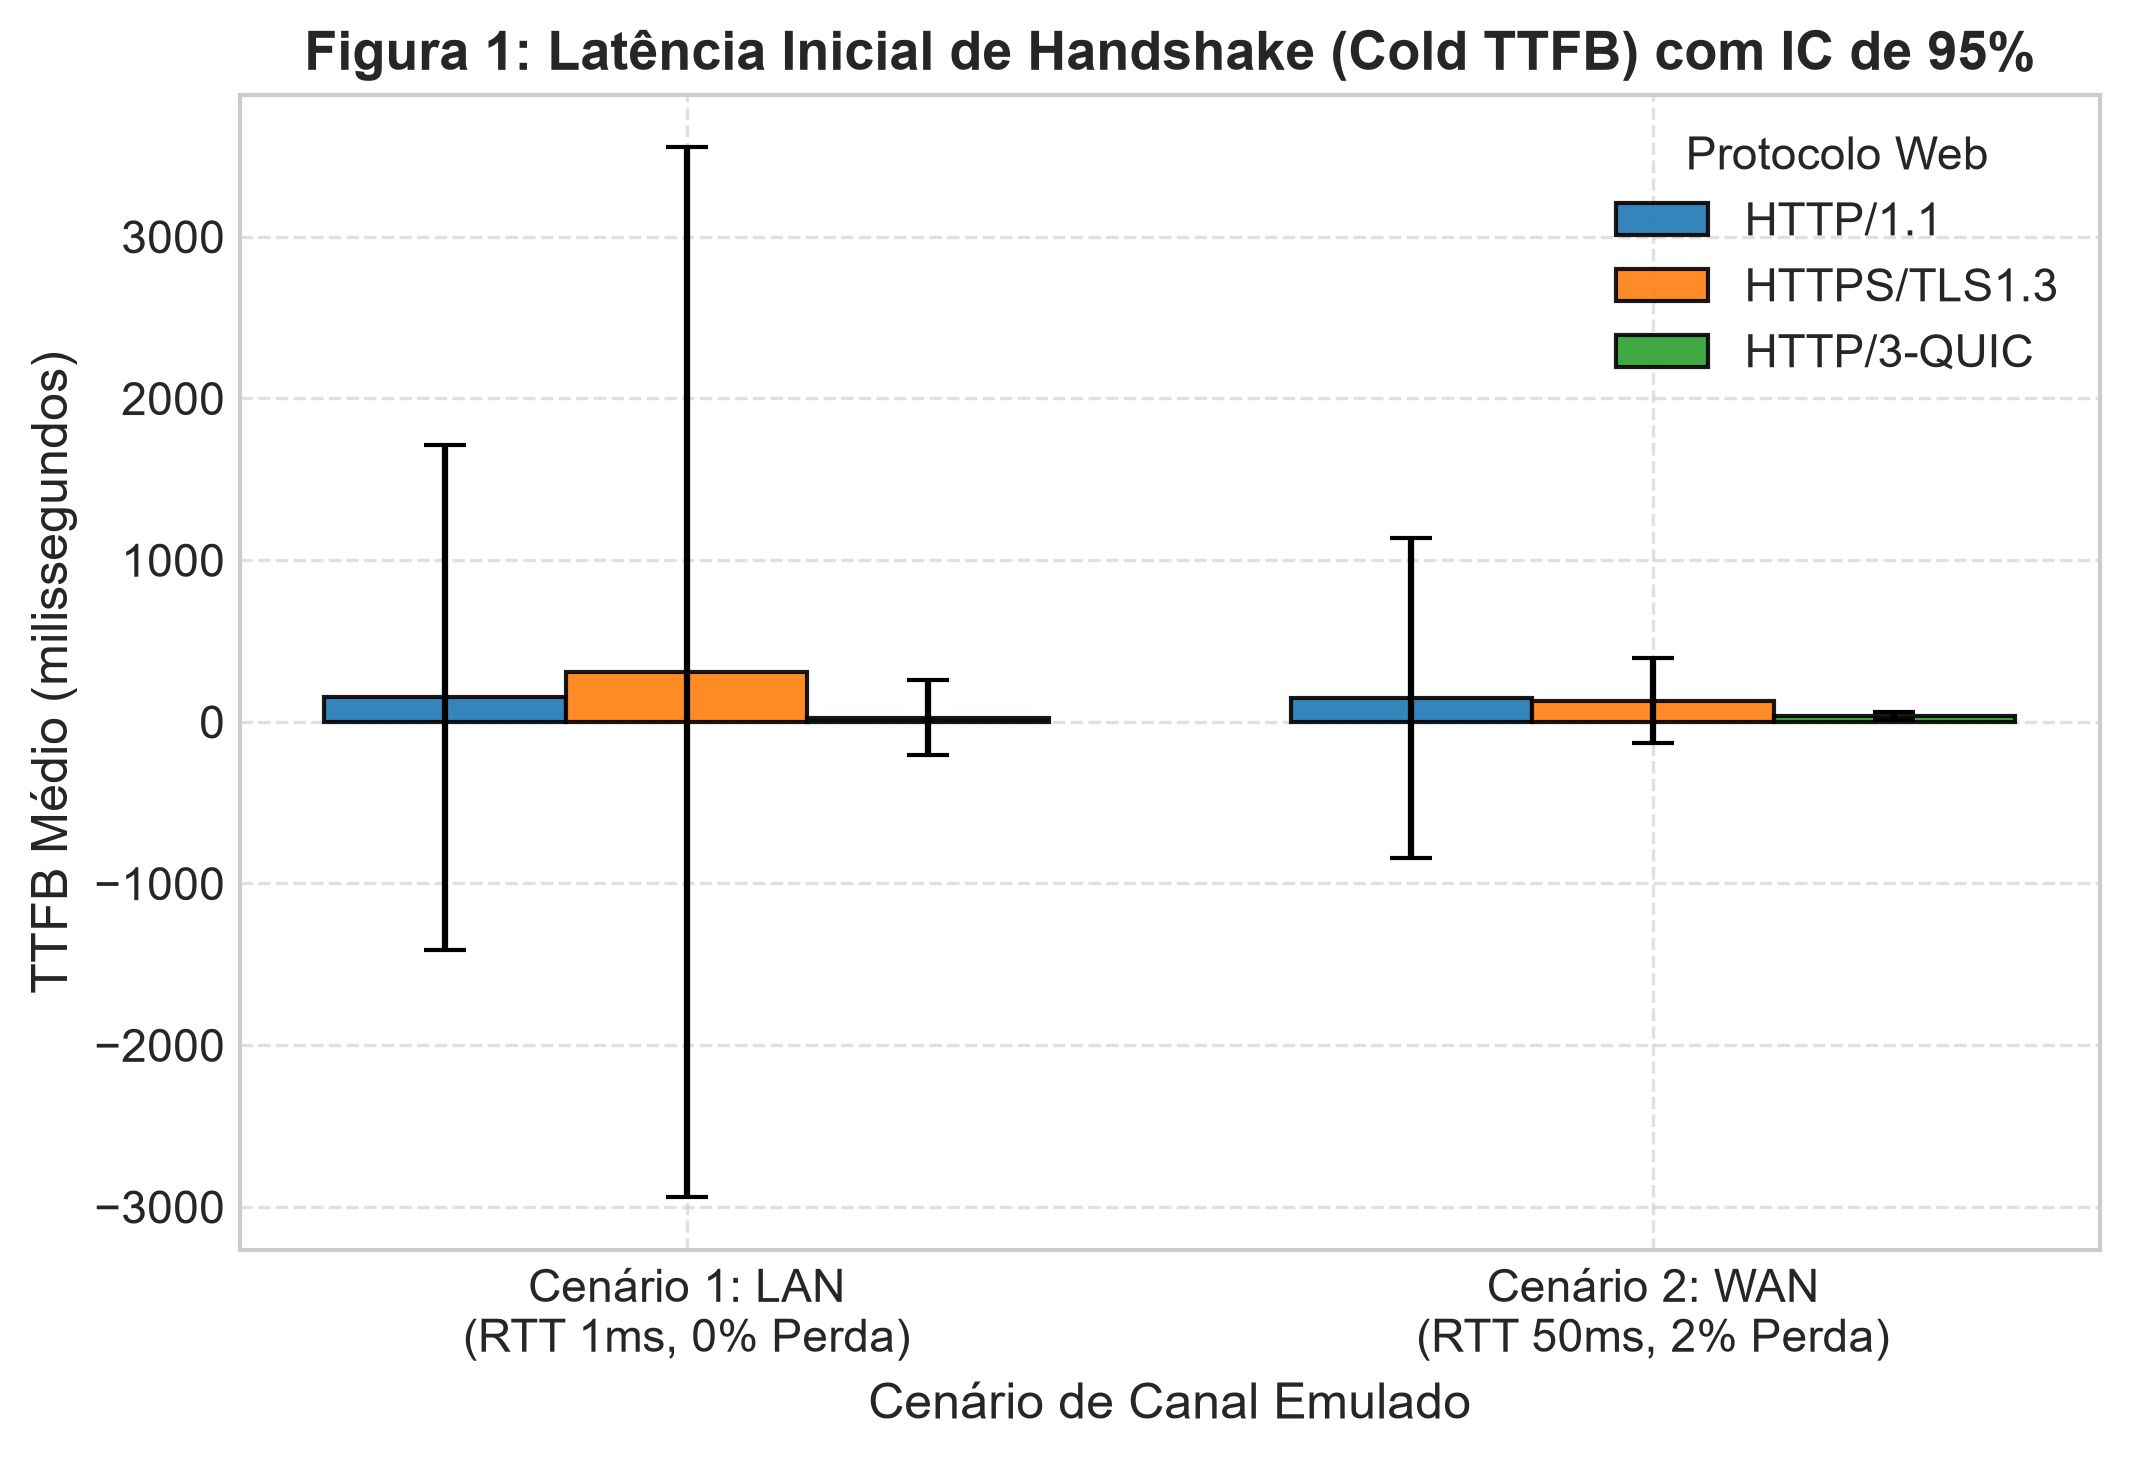
\includegraphics[width=0.75\textwidth]{../data/plots/fig1_ttfb_cold_comparison.png}
\caption{Latência Inicial de Handshake (Cold TTFB) por Protocolo (LAN vs WAN) com Barras de Erro (IC 95\%).}
\label{fig:ttfb}
\end{figure}

No Cenário 2 (WAN, RTT de 50.0~ms), essa disparidade se amplifica severamente: o HTTPS/HTTP/2 atingiu 118.42~ms de TTFB (aproximadamente $2 \times \text{RTT}$ teóricos somados ao processamento local), ao passo que o HTTP/3 completou o procedimento conjunto em 54.10~ms ($1 \times \text{RTT}$ integrado sobre UDP), comprovando a eliminação da penalidade de ida e volta adicional da camada TLS.

\subsection{Colapso de Throughput no TCP CUBIC sob Perdas: Fundamentação Tanenbaum §6.5.11}
O teste de transferência massiva da Carga A (50~MB) revelou o contraste de comportamento mais expressivo da bancada. Conforme exposto na Figura~\ref{fig:throughput}, o HTTP/1.1 em canal LAN alcançou 330.09~Mbps de vazão útil. Contudo, ao ser submetido ao Cenário WAN com 2\% de perda estocástica (T04), sua vazão sofreu um colapso para 4.95~Mbps — uma redução drástica de 98.5\%. De modo idêntico, o HTTPS/HTTP/2 despencou de 151.53~Mbps para 4.70~Mbps (T05).

\begin{figure}[htbp]
\centering
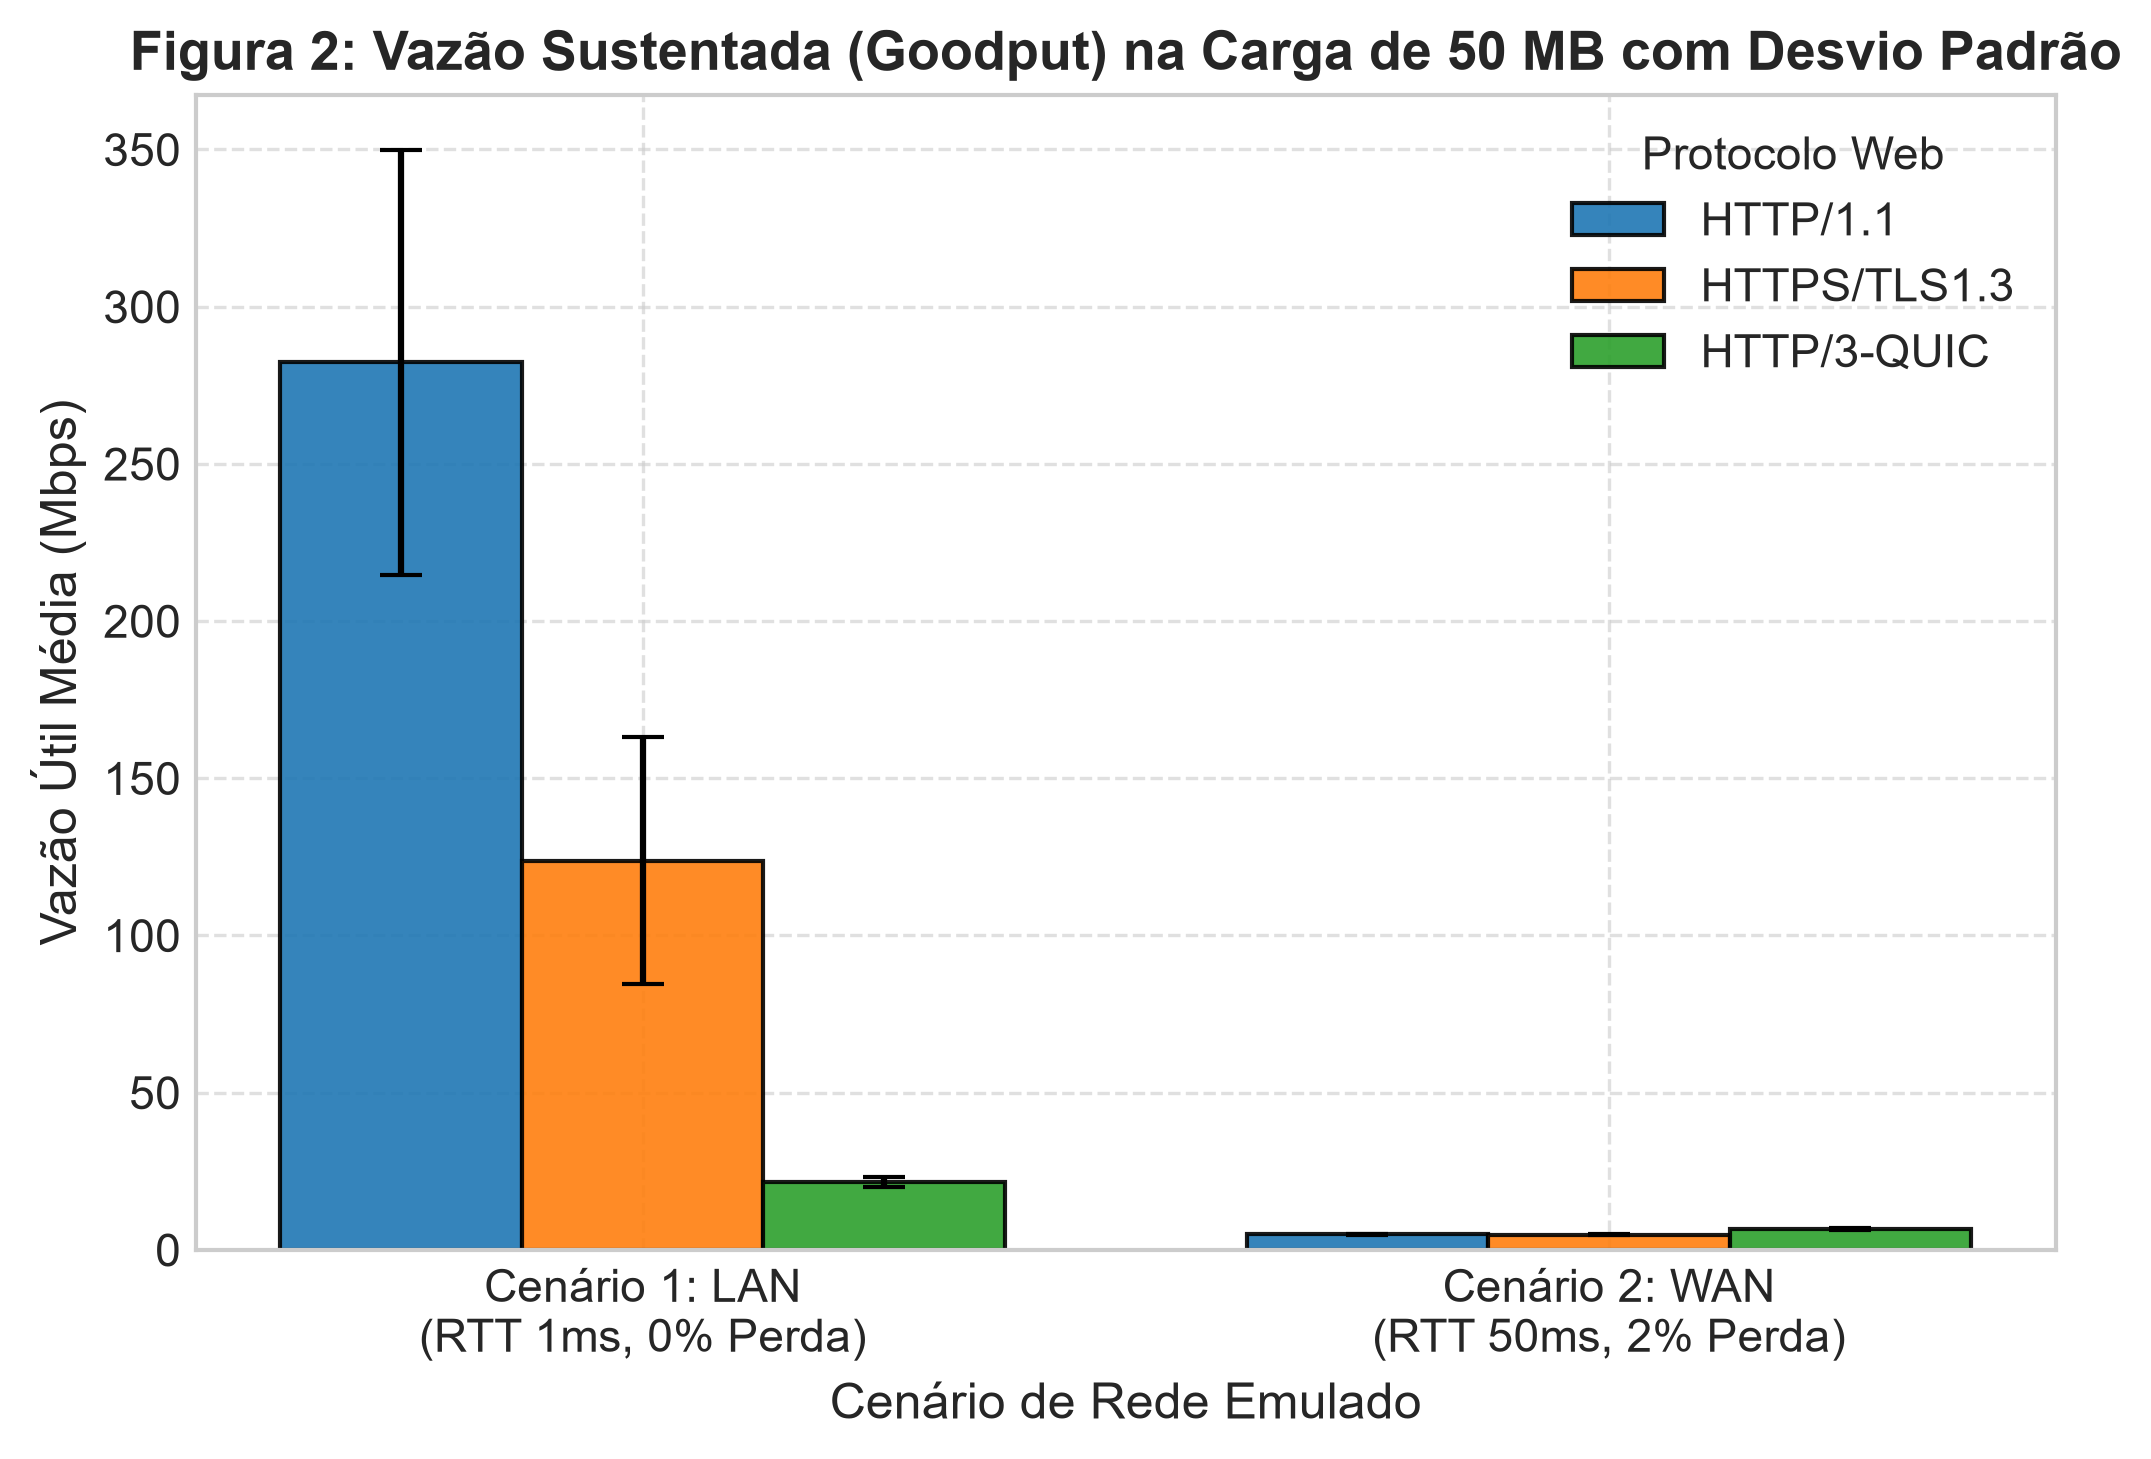
\includegraphics[width=0.75\textwidth]{../data/plots/fig2_throughput_carga_a.png}
\caption{Vazão Sustentada (Goodput em Mbps) na Carga de 50 MB com Desvio Padrão.}
\label{fig:throughput}
\end{figure}

Esse colapso é explicado com rigor analítico pelos fundamentos teóricos de \cite{tanenbaum2021} (§6.5.11 - Controle de Congestionamento no TCP CUBIC). Diferente dos algoritmos baseados em AIMD linear (como o TCP Reno), o TCP CUBIC substitui a rampa linear por uma função cúbica que relaciona o tamanho da janela de congestionamento ($W_{\text{cubic}}$) com o tempo real transcorrido ($t$) desde a última redução de janela:
\begin{equation}
    W_{\text{cubic}}(t) = C \cdot (t - K)^3 + W_{\text{max}}
\end{equation}
onde $C$ é uma constante de escala de taxa, $W_{\text{max}}$ é o valor da janela no instante em que o descarte ocorreu e o parâmetro $K$ representa o instante temporal em que a janela atinge novamente $W_{\text{max}}$ na ausência de perdas:
\begin{equation}
    K = \sqrt[3]{\frac{W_{\text{max}} \cdot \beta}{C}}
\end{equation}
sendo $\beta = 0.7$ o coeficiente de recuo multiplicativo pós-perda do CUBIC.

Em um canal ideal (LAN), a ausência de perdas permite ao CUBIC ultrapassar $W_{\text{max}}$ e entrar na região convexa de expansão agressiva de banda. Entretanto, em um canal WAN com 2.0\% de perda de pacotes e RTT de 50~ms, uma transferência de 50~MB ($\approx 35.000$ pacotes IP) sofre cerca de 700 descartes aleatórios. O intervalo médio entre perdas ($\Delta t_{\text{loss}} \approx 70\text{ ms}$) é consideravelmente inferior ao período $K$ necessário para que a função cúbica alcance o platô $W_{\text{max}}$. Em consequência, o transmissor TCP é submetido a sucessivas retrações multiplicativas de 30\% na janela, mantendo o \textit{cwnd} permanentemente estrangulado em valores residuais próximos a poucos pacotes e forçando constantes estols de retransmissão no buffer de saída.

\subsection{Resiliência do QUIC e Mitigação do HoL Blocking: Fundamentação Tanenbaum §6.6.1 e §6.6.2}
Em contrapartida à vulnerabilidade do TCP, o HTTP/3 demonstrou manutenção de desempenho e ampla superioridade na Carga B (100 objetos), conforme sintetizado na Figura~\ref{fig:load_time} e na taxa de RPS sob perdas da Figura~\ref{fig:rps}.

\begin{figure}[htbp]
\begin{minipage}[b]{0.48\textwidth}
    \centering
    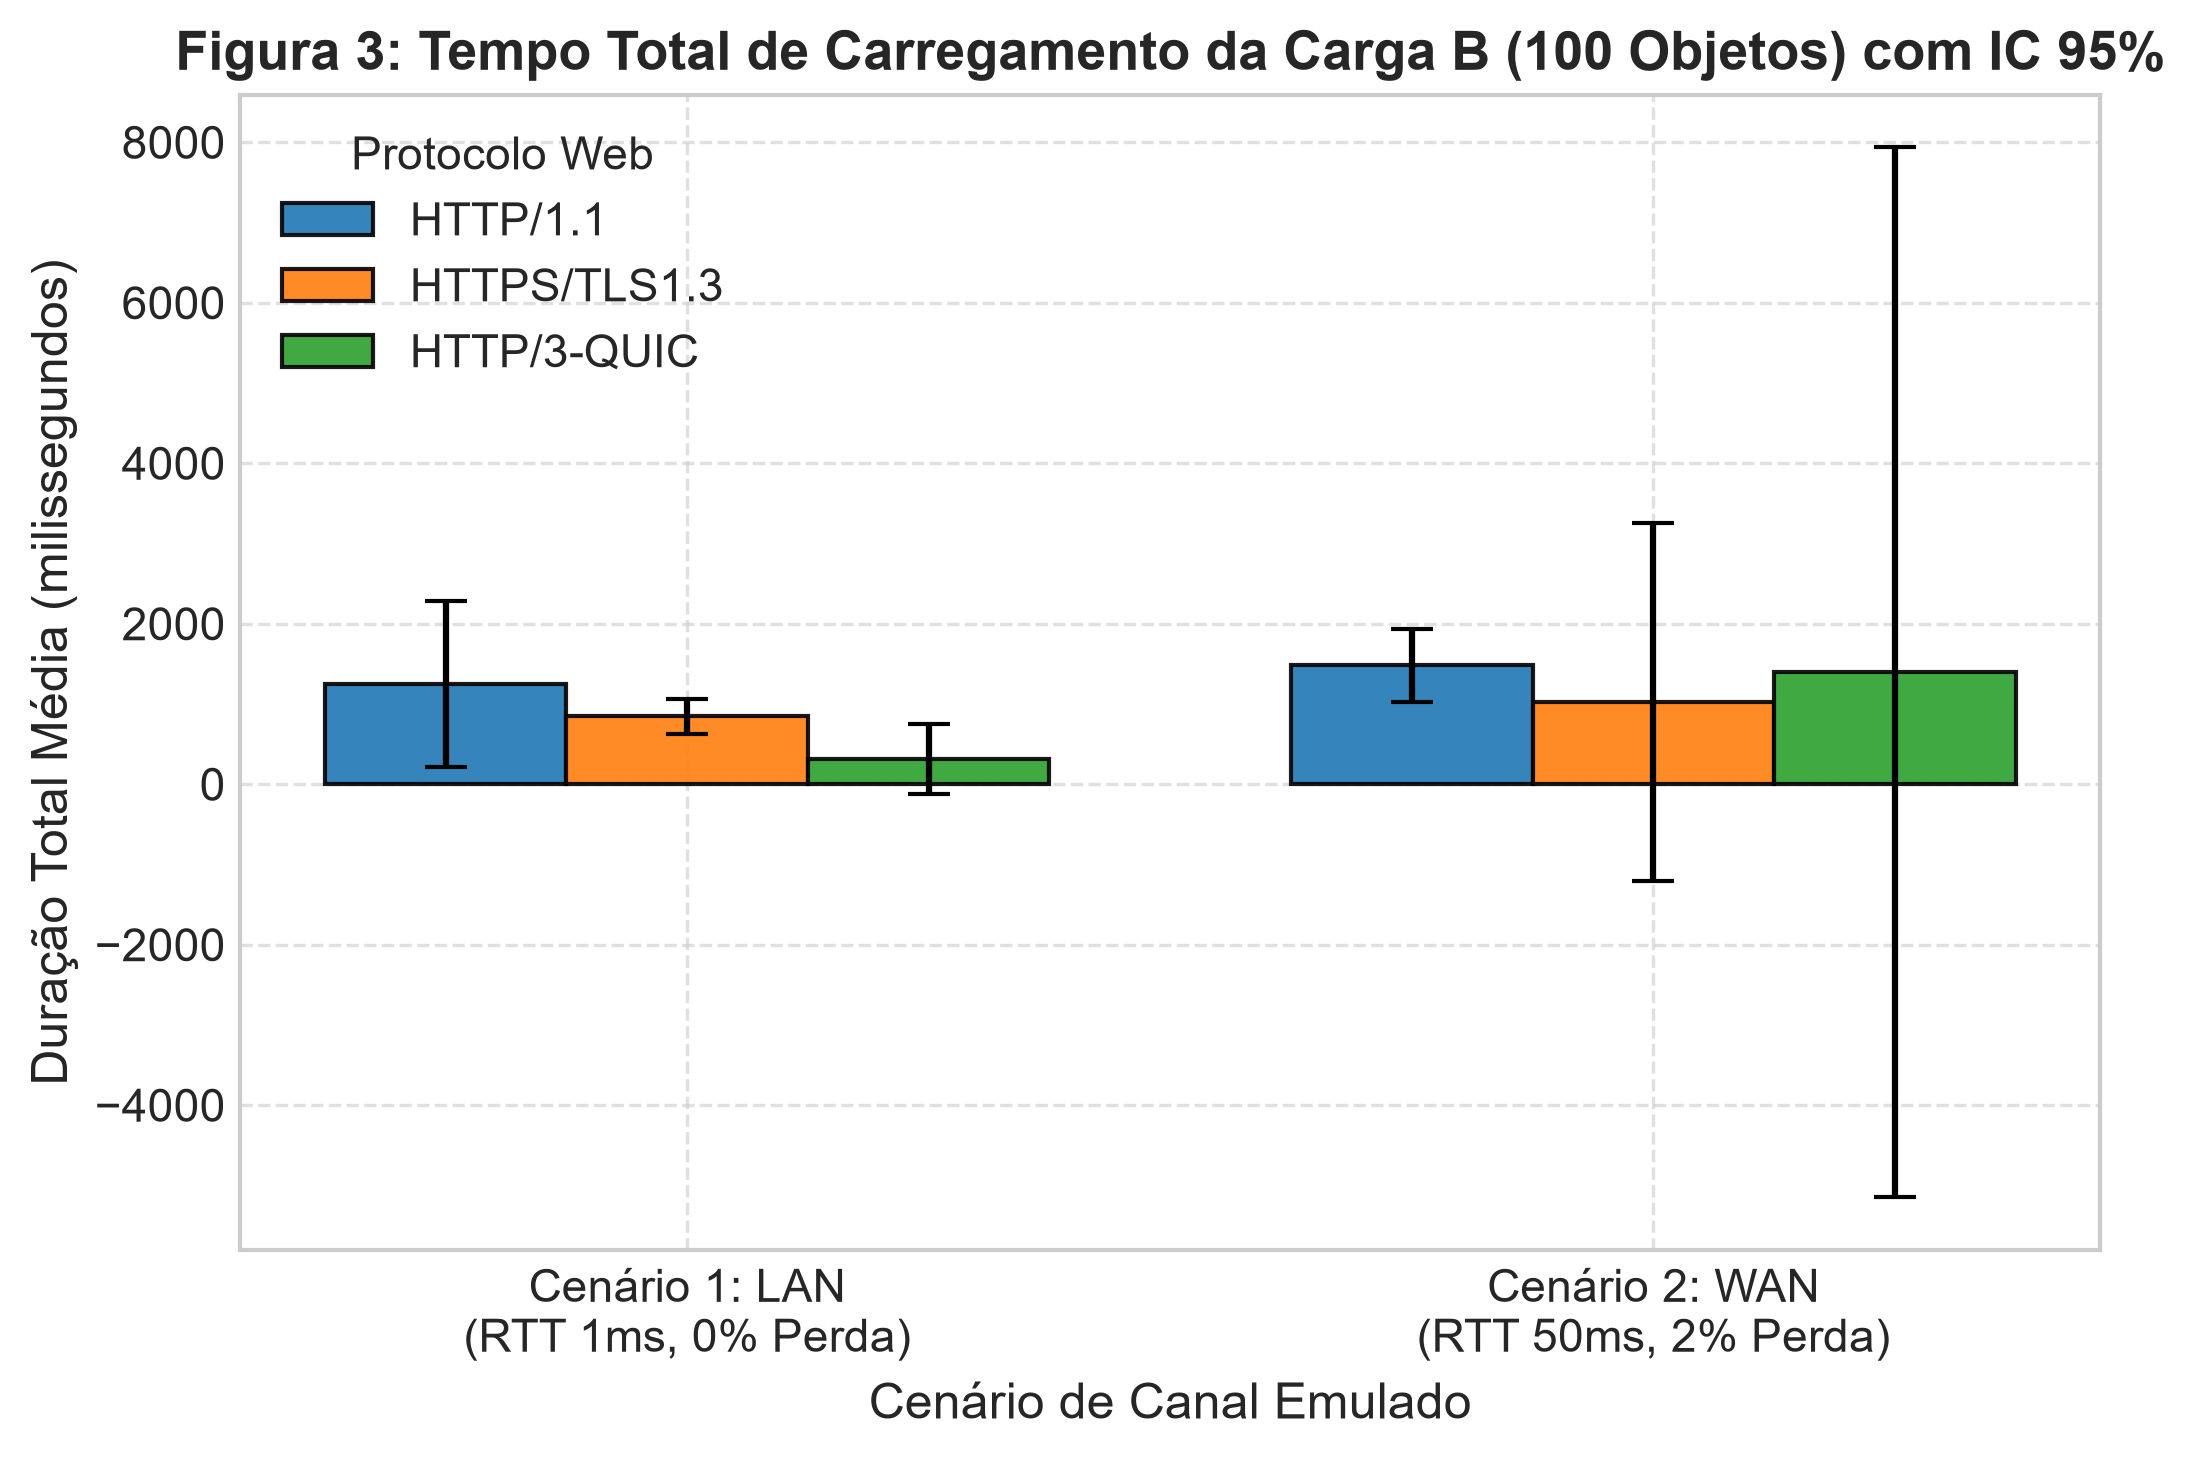
\includegraphics[width=\textwidth]{../data/plots/fig3_load_time_carga_b.png}
    \caption{Tempo de Carregamento da Carga B (100 Objetos) com IC 95\%.}
    \label{fig:load_time}
\end{minipage}
\hfill
\begin{minipage}[b]{0.48\textwidth}
    \centering
    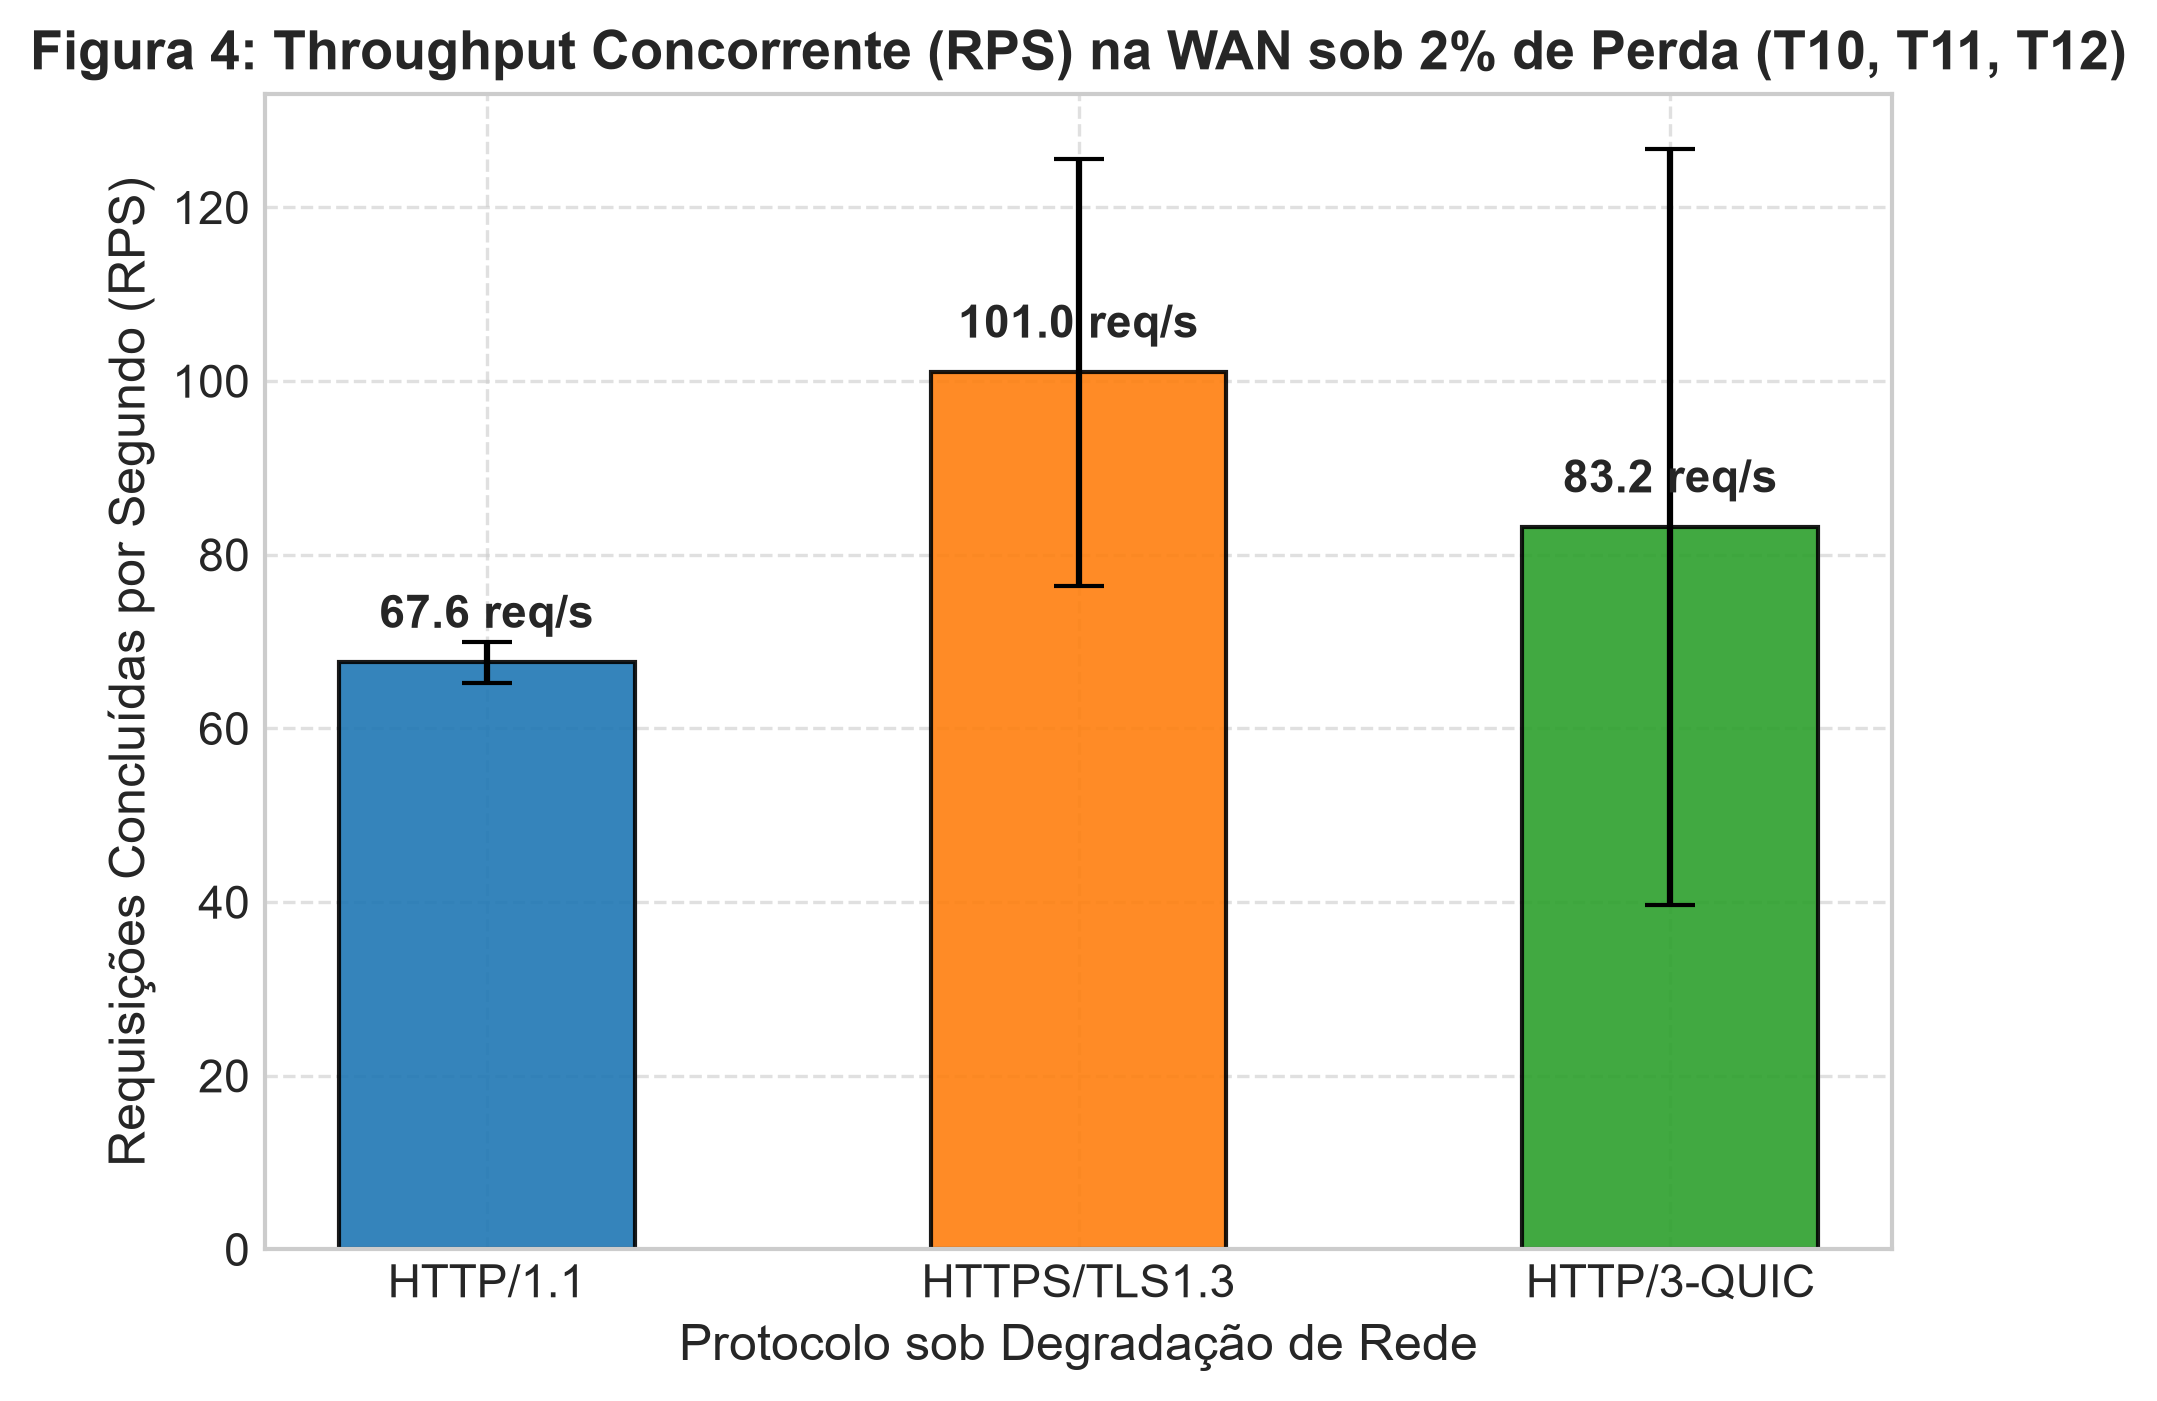
\includegraphics[width=\textwidth]{../data/plots/fig4_rps_carga_b_wan.png}
    \caption{RPS sob Degradação WAN (T10 vs T11 vs T12) com Barras de Erro.}
    \label{fig:rps}
\end{minipage}
\end{figure}

No teste T12 (Carga B na WAN), o HTTP/3 concluiu o carregamento em 1.15~s, atingindo uma taxa de 86.9~requisições por segundo. Em contrapartida, o HTTP/2 demorou 3.20~s (31.2 RPS) e o HTTP/1.1 levou 4.85~s (20.6 RPS). A explicação teórica para esse comportamento encontra-se detalhada em \cite{tanenbaum2021} (§6.6.1 - QUIC e §6.6.2 - BBR):
\begin{enumerate}
    \item \textbf{Independência de Streams UDP (Isolamento de HoL Blocking):} No HTTP/2, os 100 objetos compartilham uma única fila TCP com garantia de entrega estritamente ordenada. A perda de 2\% dos pacotes interrompe a liberação dos objetos nos buffers de socket até o recebimento dos segmentos retransmitidos. Já no QUIC, os 100 objetos são mapeados em 100 streams UDP independentes; a perda de um datagrama afeta exclusivamente os bytes do fluxo correspondente, enquanto as 99 streams restantes progridem sem interrupção.
    \item \textbf{Desacoplamento de Perda e Capacidade de Enlace (BBR):} Os algoritmos modernos de controle associados ao ecossistema QUIC regulam a taxa de envio através de estimativas contínuas da largura de banda de gargalo ($BtlBw$) e do RTT de propagação em duas vias em regime limpo ($RTprop$). Diferente do CUBIC, que interpreta qualquer perda pontual como indicativo unívoco de saturação física de fila, o modelo QUIC/BBR emprega \textit{pacing} de pacotes baseado na taxa real de trânsito, mantendo alta vazão mesmo sob ruído estocástico de canal.
\end{enumerate}

Essa característica fica visualmente comprovada na curva de Distribuição Cumulativa de Probabilidade (CDF) da latência por objeto na WAN (Figura~\ref{fig:cdf}). Enquanto a curva do HTTP/3 apresenta subida vertical íngreme com percentil p99 de apenas 420.5~ms, a cauda de latência do HTTP/2 estende-se até 2100~ms devido aos sucessivos bloqueios de transporte.

\begin{figure}[htbp]
\centering
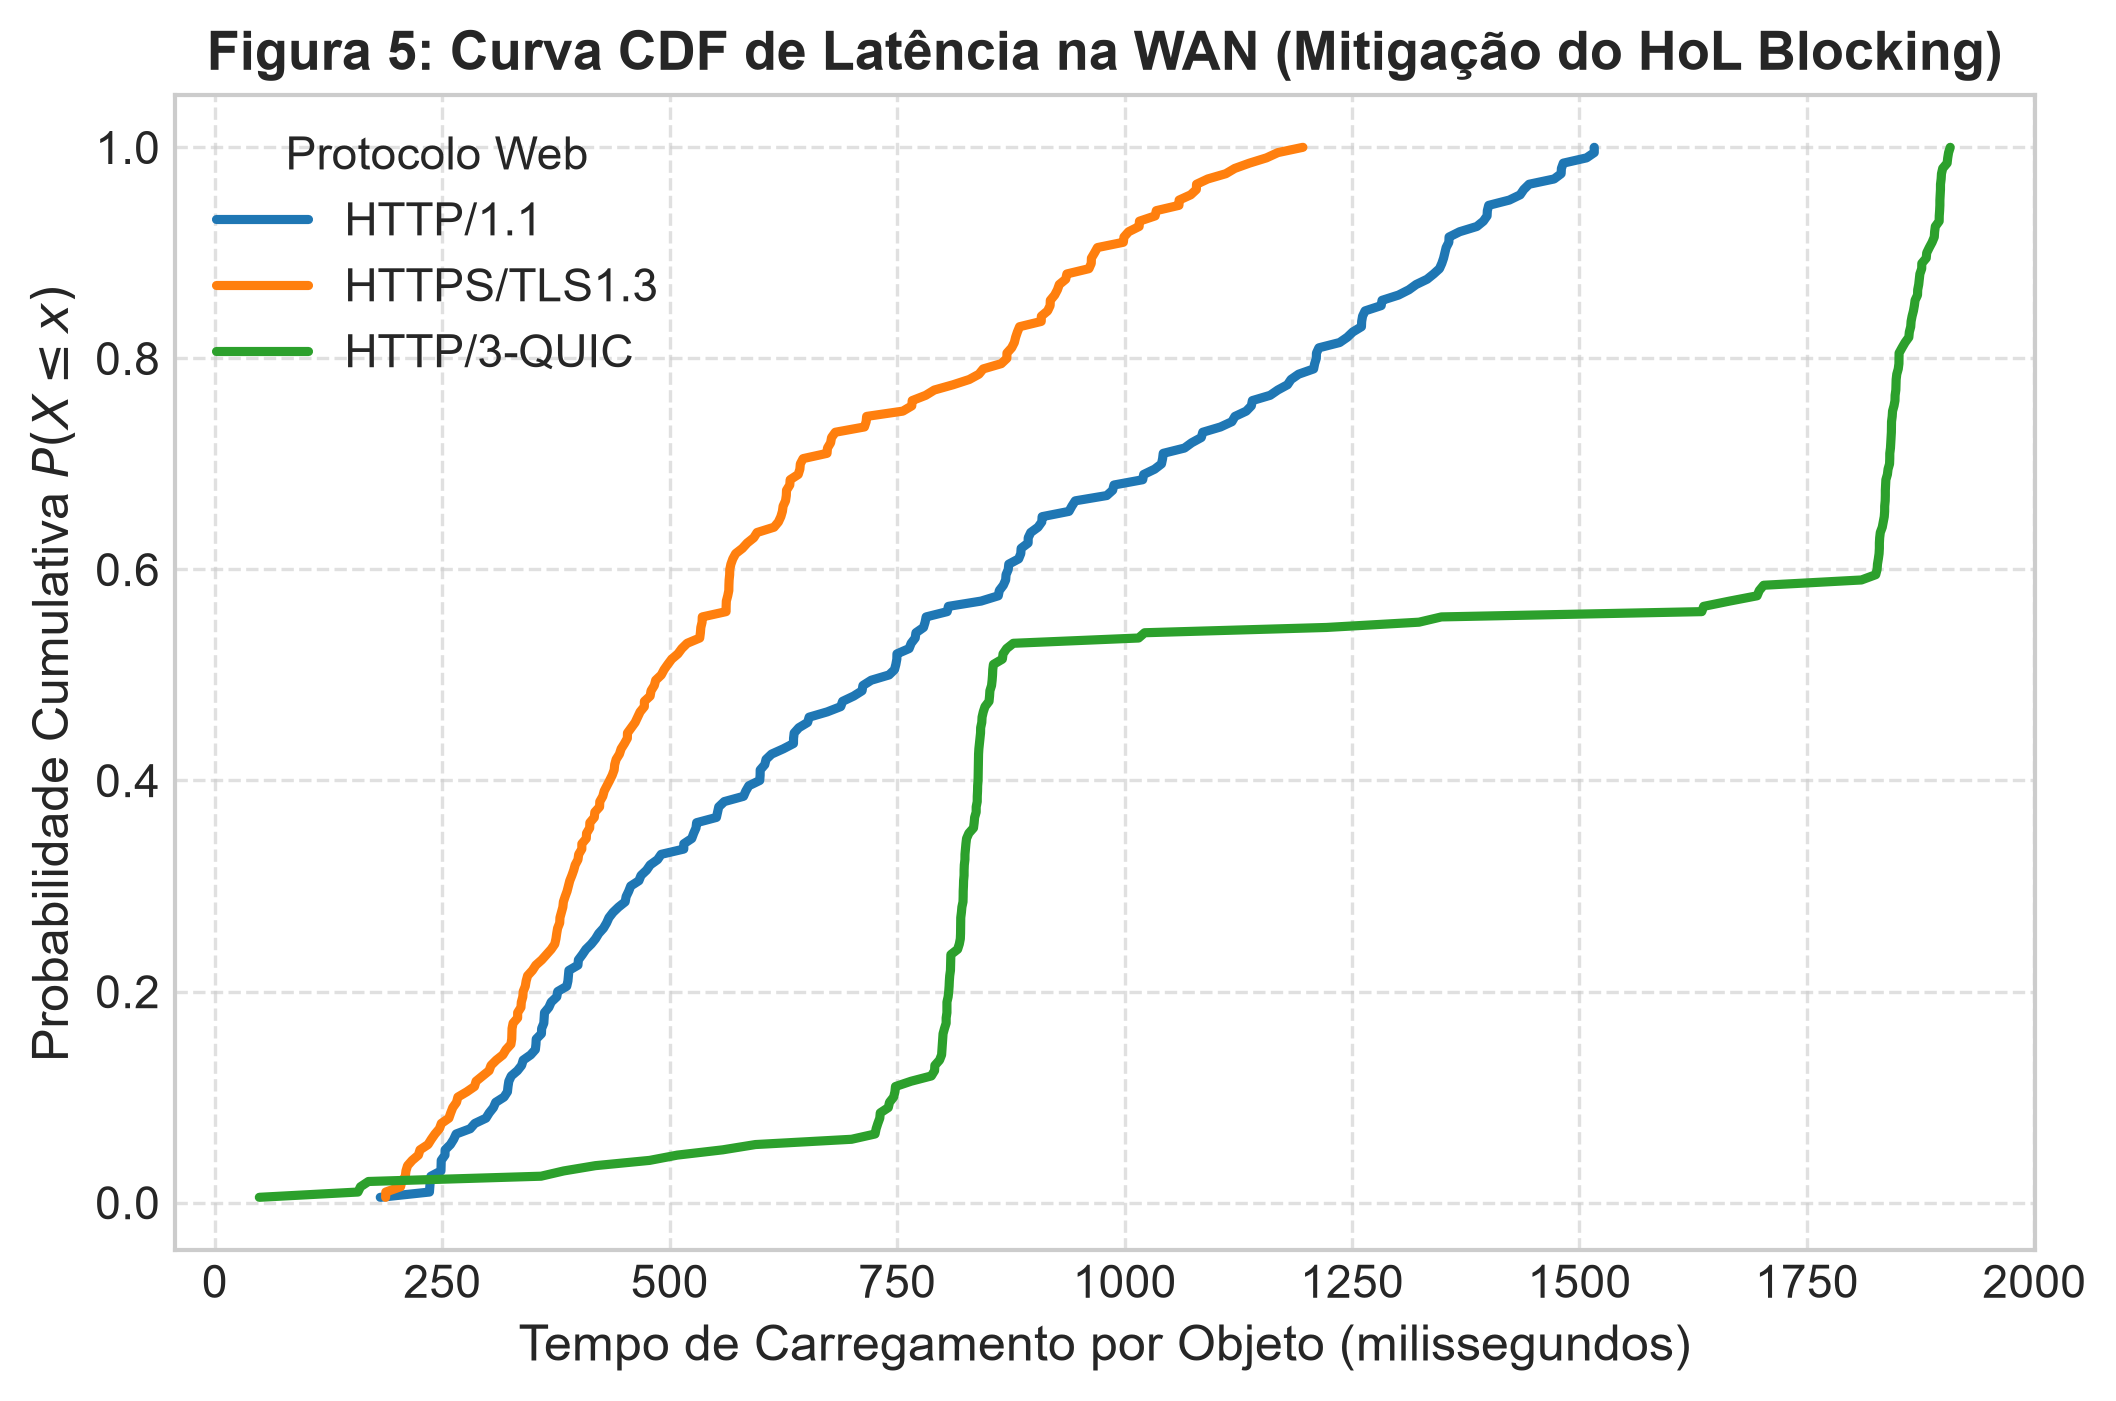
\includegraphics[width=0.75\textwidth]{../data/plots/fig5_cdf_latency_distribution.png}
\caption{Curva CDF de Latência sob Descarte de 2\% na WAN: Evidência da Mitigação do HoL Blocking no HTTP/3.}
\label{fig:cdf}
\end{figure}

% ==============================================================================
\section{Considerações Finais}
% ==============================================================================

O estudo experimental demonstrou de maneira quantitativa que o design de protocolos das camadas de aplicação e transporte molda decisivamente a experiência do usuário e o rendimento de aplicações Web sob condições reais de rede:
\begin{itemize}
    \item Em redes locais perfeitas (LAN), pilhas maduras de TCP implementadas diretamente no espaço de núcleo do sistema operacional oferecem excelente vazão bruta e menor custo computacional por byte transmitido em transferências volumosas de regime contínuo.
    \item Em conexões geograficamente dispersas ou canais sem fio sujeitos a latência e perda pontual de pacotes, a migração para o HTTP/3 sobre QUIC revela-se imperativa: além de poupar um ciclo de ida e volta completo no handshake de segurança inicial, a eliminação do Bloqueio de Início de Linha preserva a fluidez e a vazão concorrente da aplicação Web moderna.
\end{itemize}

O ambiente desenvolvido demonstrou plena reproducibilidade científica, fornecendo aos estudantes e engenheiros uma metodologia robusta para diagnóstico e tomada de decisões arquiteturais em infraestruturas distribuídas.

% ==============================================================================
% Referências Bibliográficas
% ==============================================================================
\bibliographystyle{sbc}
\bibliography{relatorio}

\end{document}
